\chapter{Heat Conduction}\label{ch:b2:heat-conduction}

Touch a metal rail and a wooden bench on the same cold morning: the
rail feels colder, though a thermometer gives both the same
temperature. Put a pan on the stove and its handle warms only after a
while; dig two metres down in summer and the soil is still cold from
the winter; a processor that dissipates a hundred watts on a square
centimetre does not melt because a block of finned aluminium sits on
it. All of this is \emph{heat conduction}, the transport of internal
energy through matter by the agitation of its molecules, without any
flow of matter --- and all of it obeys one law, Fourier's, and one
equation, the heat equation, which is the \omterm{thm:b2:particle-diffusion:equation}{diffusion equation} of the
last chapter with temperature in place of density. This chapter sets
up the law and the equation from an energy balance, solves them in the
cases that matter (stationary walls and their \omterm{prop:b2:heat-conduction:resistance}{thermal resistances},
periodic heating and the thermal wave, cooling fins), introduces the
exchange with a fluid (Newton's law and the \omterm{def:b2:heat-conduction:biot}{Biot number}), and computes
the entropy that conduction creates --- for heat flows only downhill.

\begin{omfigure}
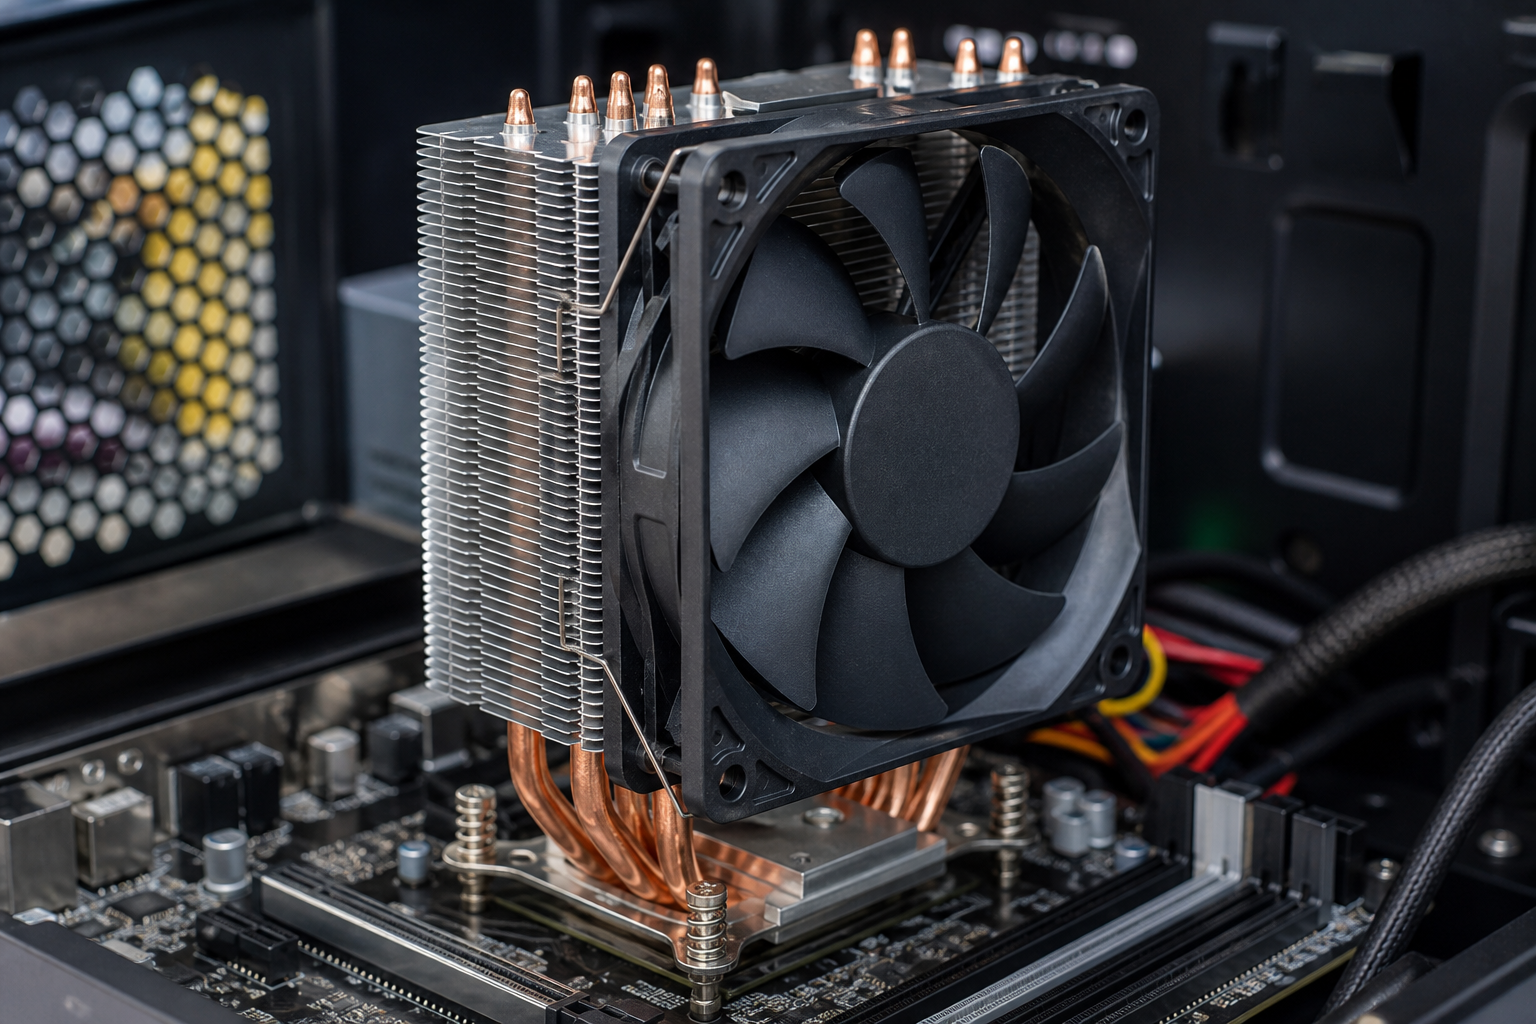
\includegraphics[width=0.58\linewidth]{images/book4/ai/b4-25-cpu-heat-sink.png}

{\small A finned heat sink on a processor: a hundred watts conducted
out of a square centimetre of silicon, spread through a metal base,
and handed to the air by fins that multiply the surface thirty times.}
\end{omfigure}

\section{Fourier's law}

\begin{definition}[Heat current density]\label{def:b2:heat-conduction:flux}
The \emph{heat current density}\index{heat current density}
$\vect{j}_Q$ (in \unit{W/m^2}) is the vector such that the energy
transferred by conduction through an oriented surface element
$\dd\vect S$ during $\dd t$ is $\vect{j}_Q\cdot\dd\vect S\,\dd t$; the
\emph{thermal flux}\index{thermal flux} (a power, in watts) through a
surface $S$ is $\Phi = \iint_S\vect{j}_Q\cdot\dd\vect S$.
\end{definition}

\begin{theorem}[Fourier's law]\label{thm:b2:heat-conduction:fourier}
In a medium at rest whose temperature is not uniform,
\[
\vect{j}_Q = -\lambda\,\vect{\operatorname{grad}}\,T ,
\]
where the \emph{thermal conductivity}\index{thermal conductivity}
$\lambda > 0$ (in \unit{W/m/K}) depends on the material and, weakly, on
the temperature. Heat flows down the temperature \omterm{def:b2:maxwell-equations:operators}{gradient}, from hot to
cold --- the second law built into a linear law.
\end{theorem}

\begin{proof}
Phenomenological, like Fick's law, and with the same microscopic
justification: the molecules (or the free electrons of a metal, or the
lattice vibrations) carry their energy on a random walk, and more of
it comes from the hot side.
\end{proof}

\begin{example}[Conductivities]\label{ex:b2:heat-conduction:values}
Metals (electrons carry the heat as well as the current ---
conductivities track each other): copper \qty{400}{W/m/K}, aluminium
\qty{240}{W/m/K}, steel \qty{50}{W/m/K}. Insulating solids: concrete
\qty{1.5}{W/m/K}, glass \qty{1}{W/m/K}, brick \qty{0.8}{W/m/K}, wood
\qty{0.15}{W/m/K}. Liquids: water \qty{0.6}{W/m/K}. Gases: air
\qty{0.026}{W/m/K} --- and the best insulators, glass wool or foam at
\qty{0.04}{W/m/K}, are mostly still air, trapped so that it cannot
convect. Four orders of magnitude from copper to air.
\end{example}

\section{The energy balance and the heat equation}

\begin{theorem}[Local energy balance]\label{thm:b2:heat-conduction:balance}
In a solid (or a fluid at rest) of density $\rho$ and specific heat
$c$, with a power $p$ released per unit volume (Joule heating, a
chemical or nuclear reaction, absorbed radiation),
\[
\rho c\,\frac{\partial T}{\partial t} = -\operatorname{div}\vect{j}_Q + p ,
\qquad\text{in one dimension}\quad
\rho c\,\frac{\partial T}{\partial t} = -\frac{\partial j_Q}{\partial x} + p .
\]
\end{theorem}

\begin{proof}
First law for the slab between $x$ and $x + \dd x$ (section $S$,
fixed volume, so no work): its internal energy $\rho c\,T\,S\,\dd x$
changes in $\dd t$ by the heat received, $[j_Q(x) - j_Q(x+\dd x)]S\,\dd t
= -\partial_x j_Q\,\dd x\,S\,\dd t$, plus $p\,S\,\dd x\,\dd t$. In three
dimensions the heat entering a fixed volume through its closed surface
is $-\iint\vect{j}_Q\cdot\dd\vect S = -\iiint\operatorname{div}\vect{j}_Q\,\dd\tau$.
\end{proof}

\begin{theorem}[Heat equation]\label{thm:b2:heat-conduction:equation}
For uniform $\lambda$, $\rho$, $c$,
\[
\frac{\partial T}{\partial t} = a\,\Delta T + \frac{p}{\rho c},
\qquad a = \frac{\lambda}{\rho c} \quad\text{(the \emph{thermal diffusivity}\index{thermal diffusivity}, in \unit{m^2/s})} .
\]
Everything said of the \omterm{thm:b2:particle-diffusion:equation}{diffusion equation} holds: linearity,
irreversibility, smoothing, and the scales $L \sim \sqrt{at}$, $t \sim
L^2/a$.
\end{theorem}

\begin{proof}
Insert Fourier's law in the balance: $\rho c\,\partial_t T =
\lambda\Delta T + p$.
\end{proof}

\begin{example}[Diffusivities and times]\label{ex:b2:heat-conduction:times}
Copper $a = \qty{1.1e-4}{m^2/s}$, air \qty{2e-5}{m^2/s}, concrete and
brick $\approx \qty{5e-7}{m^2/s}$, water \qty{1.4e-7}{m^2/s}, wood
\qty{1e-7}{m^2/s}. Heat crosses a centimetre of copper in a second, a
centimetre of brick in three minutes, a \qty{20}{cm} wall in a day
(which is why thick walls smooth the day--night cycle), the
\qty{1.5}{cm} half-thickness of a steak in a quarter of an hour (cooking
times scale as the square of the thickness), and a kilometre of rock
in $10^{12}\,\unit{s}$, thirty thousand years --- the Earth is still
cooling from its formation.
\end{example}

\section{Stationary regime: thermal resistances}

\begin{proposition}[Thermal resistance of a slab]\label{prop:b2:heat-conduction:resistance}
In the stationary regime without sources, a slab of thickness $e$,
area $S$, conductivity $\lambda$, between the temperatures $T_1$ and
$T_2$, has a linear profile and carries the flux
\[
\Phi = \frac{T_1 - T_2}{R_{\text{th}}}, \qquad
R_{\text{th}} = \frac{e}{\lambda S}\quad\text{(in \unit{K/W})} :
\]
its \emph{thermal resistance}\index{thermal resistance}. Temperature
plays the role of potential, the flux that of current: resistances in
series (layers of a wall) add, resistances in parallel (wall and
window) add their inverses. For a cylindrical shell (a pipe's
insulation) between the radii $r_1 < r_2$ and of length $\ell$,
$R_{\text{th}} = \ln(r_2/r_1)/2\pi\lambda\ell$; for a spherical shell,
$(1/r_1 - 1/r_2)/4\pi\lambda$.
\end{proposition}

\begin{proof}
$\dd^2T/\dd x^2 = 0$: affine profile, $j_Q = \lambda(T_1 - T_2)/e$
uniform, $\Phi = j_QS$. In cylindrical geometry $\Phi = -\lambda\,2\pi
r\ell\,\dd T/\dd r$ is the same at every $r$ (no accumulation), so
$T = A - (\Phi/2\pi\lambda\ell)\ln r$; in spherical geometry, $\Phi =
-4\pi r^2\lambda\,\dd T/\dd r$ gives $T = A + \Phi/4\pi\lambda r$.
\end{proof}

\begin{proposition}[Exchange with a fluid: Newton's law]\label{prop:b2:heat-conduction:newton}
A solid surface at $T_{\text{s}}$ in contact with a fluid at $T_{\text{f}}$
(away from the surface) loses the flux density
\[
j_Q = h\,(T_{\text{s}} - T_{\text{f}}) ,
\]
where the \emph{heat transfer coefficient}\index{heat transfer
coefficient} $h$ (in \unit{W/m^2/K}) sums up the conduction through
the thin fluid layer that sticks to the wall and the convection that
renews it: $h \approx 5$--\qty{25}{W/m^2/K} for air in natural or
light convection, $50$--\qty{500}{W/m^2/K} for forced air, $10^3$--$10^4$
for water. The surface then adds a \emph{film resistance} $1/hS$ in
series with the wall.
\end{proposition}

\begin{proof}
Phenomenological: the fluid's motion is not computed, it is summarised
in $h$ (measured, or given by the correlations of fluid mechanics).
\end{proof}

\begin{omfigure}
\begin{tikzpicture}[scale=0.9, >=stealth]
  % wall layers
  \fill[omExo!15] (0,0) rectangle (1.6,2.6);
  \fill[omDef!12] (1.6,0) rectangle (2.6,2.6);
  \fill[gray!15] (2.6,0) rectangle (2.8,2.6);
  \draw (0,0) rectangle (2.8,2.6);
  \draw (1.6,0) -- (1.6,2.6); \draw (2.6,0) -- (2.6,2.6);
  \node[font=\scriptsize] at (0.8,2.85) {brick};
  \node[font=\scriptsize] at (2.1,2.85) {wool};
  \node[font=\scriptsize, right] at (2.9,1.3) {inside $T_{\text{i}}$};
  \node[font=\scriptsize, left] at (-0.1,1.3) {outside $T_{\text{o}}$};
  \draw[->, omThm, thick] (3.6,0.7) -- (-0.8,0.7) node[midway, below, font=\scriptsize] {$\Phi$};
  % resistor chain
  \begin{scope}[yshift=-1.6cm]
    \draw (-0.8,0) -- (0.2,0);
    \draw (0.2,-0.18) rectangle (1.0,0.18); \node[font=\tiny] at (0.6,0) {$1/h_{\text{o}}S$};
    \draw (1.0,0) -- (1.4,0);
    \draw (1.4,-0.18) rectangle (2.4,0.18); \node[font=\tiny] at (1.9,0) {$e_1/\lambda_1 S$};
    \draw (2.4,0) -- (2.8,0);
    \draw (2.8,-0.18) rectangle (3.8,0.18); \node[font=\tiny] at (3.3,0) {$e_2/\lambda_2 S$};
    \draw (3.8,0) -- (4.2,0);
    \draw (4.2,-0.18) rectangle (5.0,0.18); \node[font=\tiny] at (4.6,0) {$1/h_{\text{i}}S$};
    \draw (5.0,0) -- (5.6,0);
    \fill (-0.8,0) circle (1.5pt) node[above, font=\scriptsize] {$T_{\text{o}}$};
    \fill (5.6,0) circle (1.5pt) node[above, font=\scriptsize] {$T_{\text{i}}$};
  \end{scope}
  % profile
  \begin{scope}[xshift=7.2cm]
    \draw[->] (0,0) -- (3.4,0) node[right, font=\scriptsize] {$x$};
    \draw[->] (0,0) -- (0,2.8) node[above, font=\scriptsize] {$T$};
    \draw[omDef, thick] (0,0.4) -- (0.3,0.6) -- (1.6,0.9) -- (2.6,2.4) -- (2.8,2.45) -- (3.2,2.6);
    \draw[dashed] (0.3,0) -- (0.3,0.6); \draw[dashed] (1.6,0) -- (1.6,0.9); \draw[dashed] (2.6,0) -- (2.6,2.4); \draw[dashed] (2.8,0) -- (2.8,2.45);
    \node[font=\scriptsize, below] at (0.95,0) {brick};
    \node[font=\scriptsize, below] at (2.1,0) {wool};
    \node[font=\scriptsize, left] at (0,0.4) {$T_{\text{o}}$};
    \node[font=\scriptsize, right] at (3.2,2.6) {$T_{\text{i}}$};
  \end{scope}
\end{tikzpicture}

{\small A composite wall and its thermal circuit: film, brick, wool,
film in series. Right: the temperature profile --- almost all the drop
falls across the layer of largest resistance, the wool, though it is
the thinnest.}
\end{omfigure}

\begin{example}[A wall and a window]\label{ex:b2:heat-conduction:wall}
Per square metre: brick \qty{20}{cm} at \qty{0.8}{W/m/K}, $R =
\qty{0.25}{m^2.K/W}$; the two films, $1/8 + 1/25 = \qty{0.165}{m^2.K/W}$:
total $0.415$, i.e. $U = 1/R = \qty{2.4}{W/m^2/K}$ and, for a \qty{20}{K}
difference, \qty{48}{W/m^2}. Add \qty{10}{cm} of glass wool, $R =
\qty{2.5}{m^2.K/W}$: the total is $2.9$, $U = \qty{0.34}{W/m^2/K}$ ---
seven times less. A single pane of glass, \qty{4}{mm} at \qty{1}{W/m/K},
is all film: $R = 0.004 + 0.165$, $U \approx \qty{6}{W/m^2/K}$; a
\qty{12}{mm} layer of still air between two panes adds $0.012/0.026 =
\qty{0.46}{m^2.K/W}$ and divides the loss by more than three.
\end{example}

\begin{definition}[Biot number]\label{def:b2:heat-conduction:biot}
For a solid of size $L$ exchanging with a fluid, the \emph{Biot
number}\index{Biot number}
\[
\mathrm{Bi} = \frac{hL}{\lambda} = \frac{\text{internal resistance } L/\lambda S}{\text{film resistance } 1/hS}
\]
compares the two. If $\mathrm{Bi} \ll 1$ the solid is uniform in
temperature at every instant and cools as a whole, exponentially with
the time constant $\tau = \rho c V/hS$; if $\mathrm{Bi} \gg 1$ the
surface is at the fluid temperature and the interior conducts at its
own pace $L^2/a$.
\end{definition}

\section{Periodic heating: the thermal wave}

\begin{proposition}[Thermal wave in a half-space]\label{prop:b2:heat-conduction:wave}
If the surface $x = 0$ of a half-space is held at $T(0,t) = T_0 +
\theta_0\cos\omega t$, the temperature inside is, in the established
regime,
\[
T(x,t) = T_0 + \theta_0\,\eu^{-x/\delta}\cos\Big(\omega t - \frac{x}{\delta}\Big),
\qquad \delta = \sqrt{\frac{2a}{\omega}} :
\]
a wave that propagates inward at the speed $\omega\delta =
\sqrt{2a\omega}$ and is damped over one \emph{penetration depth} $\delta$
per radian of phase --- by $\eu^{-2\pi} = 2 \times 10^{-3}$ per
wavelength. Fast oscillations penetrate less than slow ones.
\end{proposition}

\begin{proof}
Seek $\underline T = \theta_0\eu^{\iu(\omega t - \underline k x)}$:
$\iu\omega = -a\underline k^2$, so $\underline k^2 = -\iu\omega/a$,
$\underline k = (1 - \iu)\sqrt{\omega/2a} = (1 - \iu)/\delta$ (the root
that decays for $x > 0$). Take the real part.
\end{proof}

\begin{omfigure}
\begin{tikzpicture}
  \begin{axis}[omaxis, width=9cm, height=4.8cm, xmin=0, xmax=4.6, ymin=-1.1, ymax=1.1,
    xlabel={$x/\delta$}, ylabel={$(T - T_0)/\theta_0$}, xtick={1,2,3,4}, ytick={-1,1}, clip=false,
    axis x line=middle, axis y line=left,
    legend style={font=\scriptsize, at={(0.98,0.04)}, anchor=south east, draw=none, fill=none}]
    \addplot[omDef, thick, domain=0:4.6, samples=120] {exp(-x)*cos(deg(-x))};
    \addlegendentry{$\omega t = 0$}
    \addplot[omThm, thick, domain=0:4.6, samples=120] {exp(-x)*cos(deg(pi/2-x))};
    \addlegendentry{$\omega t = \pi/2$}
    \addplot[omExo, thick, domain=0:4.6, samples=120] {exp(-x)*cos(deg(pi-x))};
    \addlegendentry{$\omega t = \pi$}
    \addplot[gray, dashed, domain=0:4.6, samples=60] {exp(-x)};
    \addplot[gray, dashed, domain=0:4.6, samples=60] {-exp(-x)};
  \end{axis}
\end{tikzpicture}

{\small The thermal wave at three instants: the surface oscillation
penetrates as a damped wave, its amplitude falling as $\eu^{-x/\delta}$
(dashed) and its phase lagging by $x/\delta$ --- at $x = \pi\delta$ the
temperature is opposite to the surface's.}
\end{omfigure}

\begin{example}[The soil, the cellar and the wine]\label{ex:b2:heat-conduction:soil}
Soil, $a \approx \qty{5e-7}{m^2/s}$. Daily cycle, $\omega = 2\pi/\qty{86400}{s}$:
$\delta = \qty{12}{cm}$ --- half a metre down the day is gone. Annual cycle:
$\delta = \qty{2.2}{m}$; at that depth the \qty{10}{K} summer--winter swing is
down to \qty{3.7}{K} and lags by one radian, two months: the cellar is
coldest in March and warmest in September, and at \qty{5}{m} it is
\qty{1}{K} from constant --- the cellar that keeps wine. The same
mathematics gives the \omterm{def:b2:dispersion-wave-packets:complex}{skin depth} of electromagnetism
(\cref{ch:b2:waves-in-media}): same equation, same $\sqrt{2/(\text{diffusivity}
\times\omega)}$.
\end{example}

\section{Fins}

\begin{proposition}[The cooling fin]\label{prop:b2:heat-conduction:fin}
A thin rod or plate (section $S$, perimeter $p$, conductivity $\lambda$)
attached at $x = 0$ to a wall at $T_0$, in a fluid at $T_{\text{f}}$ with
the coefficient $h$, has the excess temperature $\theta = T - T_{\text{f}}$
obeying
\[
\frac{\dd^2\theta}{\dd x^2} = m^2\theta, \qquad m = \sqrt{\frac{hp}{\lambda S}} ;
\]
for a long fin, $\theta = \theta_0\eu^{-mx}$ and the fin evacuates $\Phi =
\sqrt{hp\lambda S}\,\theta_0$ --- as much as a bare surface $\sqrt{\lambda
S/hp} = 1/m$ long, with a temperature that has fallen to $\theta_0/\eu$ at
$x = 1/m$. For a fin of finite length $L$ (tip adiabatic), $\theta =
\theta_0\cosh m(L-x)/\cosh mL$ and its \emph{efficiency}\index{fin
efficiency} --- the flux over that of an isothermal fin at $\theta_0$ ---
is $\eta = \tanh(mL)/mL$.
\end{proposition}

\begin{proof}
Stationary balance of the slice $[x, x + \dd x]$: conducted in,
$-\lambda S\theta'(x)$; out, $-\lambda S\theta'(x + \dd x)$; lost to the
fluid, $hp\,\theta\,\dd x$: $\lambda S\theta'' = hp\theta$. The flux at the
base is $-\lambda S\theta'(0)$: $\lambda Sm\theta_0$ for the long fin,
$\lambda Sm\theta_0\tanh mL$ for the finite one, to be compared with
$hpL\theta_0$. The \omterm{def:b2:heat-conduction:biot}{Biot number} across the fin's thickness, $ht/\lambda$, must
be small for the one-dimensional treatment.
\end{proof}

\begin{omfigure}
\begin{tikzpicture}
  \begin{axis}[omaxis, width=6.4cm, height=4.4cm, xmin=0, xmax=3.2, ymin=0, ymax=1.12,
    xlabel={$mx$}, ylabel={$\theta/\theta_0$}, xtick={1,2,3}, ytick={1}, clip=false,
    legend style={font=\scriptsize, at={(0.98,0.98)}, anchor=north east, draw=none, fill=none}]
    \addplot[omDef, thick, domain=0:3.2, samples=60] {exp(-x)};
    \addlegendentry{long fin}
    \addplot[omExo, thick, domain=0:1.2, samples=60] {cosh(1.2-x)/cosh(1.2)};
    \addlegendentry{$mL = 1.2$}
    \addplot[omThm, thick, domain=0:0.5, samples=30] {cosh(0.5-x)/cosh(0.5)};
    \addlegendentry{$mL = 0.5$}
  \end{axis}
  \begin{scope}[xshift=7.2cm, yshift=0.3cm, scale=0.8, >=stealth]
    \fill[gray!25] (0,0) rectangle (0.5,3.2);
    \fill[omDef!20] (0.5,1.4) rectangle (4.2,1.8);
    \draw (0.5,1.4) rectangle (4.2,1.8);
    \node[font=\scriptsize, rotate=90] at (0.25,1.6) {wall $T_0$};
    \draw[->, omThm, thick] (0.6,1.6) -- (1.6,1.6) node[right, font=\scriptsize] {$-\lambda S\theta'$};
    \foreach \x in {1.2,2.0,2.8,3.6}{
      \draw[->, omExo] (\x,1.85) -- (\x,2.4);
      \draw[->, omExo] (\x,1.35) -- (\x,0.8);
    }
    \node[font=\scriptsize, omExo] at (2.4,2.7) {$hp\,\theta\,\dd x$};
    \node[font=\scriptsize] at (2.4,0.45) {fluid $T_{\text{f}}$};
  \end{scope}
\end{tikzpicture}

{\small Left: temperature along a fin, for a long fin and two finite
ones (adiabatic tip) --- beyond $mx \approx 2$ a fin adds little. Right:
the balance of a slice: conduction along, convection out through the
perimeter.}
\end{omfigure}

\begin{example}[A heat sink]\label{ex:b2:heat-conduction:sink}
Aluminium fins \qty{1}{mm} thick ($p/S \approx 2/t = \qty{2000}{m^{-1}}$),
\qty{30}{mm} high, in forced air $h = \qty{50}{W/m^2/K}$: $m =
\sqrt{2h/\lambda t} = \qty{20}{m^{-1}}$, $mL = 0.6$, $\eta = 0.89$ --- the
fins work at $89\%$ of their area. Thirty of them, \qty{60}{mm} wide,
offer \qty{0.11}{m^2} where the bare \qty{60}{mm} square offered
\qty{0.0036}{m^2}: a resistance $1/\eta hA = \qty{0.2}{K/W}$ instead of
\qty{5.6}{K/W}; \qty{100}{W} raise the base by \qty{20}{K} instead of
\qty{560}{K}. Longer fins gain little ($\tanh$ saturates), thinner ones
lose efficiency: $mL \approx 1$ is the engineer's compromise.
\end{example}

\section{Entropy created by conduction}

\begin{proposition}[Entropy production]\label{prop:b2:heat-conduction:entropy}
A flux $\Phi$ conducted from a body at $T_{\text{h}}$ to a body at
$T_{\text{c}} < T_{\text{h}}$ through a stationary wall creates entropy at
the rate
\[
\dot S_{\text{c}} = \Phi\Big(\frac{1}{T_{\text{c}}} - \frac{1}{T_{\text{h}}}\Big) > 0 ;
\]
locally, conduction creates $\sigma_s = \lambda\,(\vect{\operatorname{grad}}\,T)^2/T^2
\ge 0$ per unit volume and time --- zero only where the temperature is
uniform. Heat conduction is irreversible: the same energy, delivered at
a lower temperature, can do less work.
\end{proposition}

\begin{proof}
The wall's state does not change, so its entropy is constant: the hot
body loses $\Phi/T_{\text{h}}$ per unit time, the cold one gains
$\Phi/T_{\text{c}}$; the difference is created. Locally, the entropy
balance $\partial_t(\rho s) + \operatorname{div}(\vect{j}_Q/T) = \sigma_s$
with $\rho T\partial_t s = -\operatorname{div}\vect{j}_Q$ gives $\sigma_s =
\vect{j}_Q\cdot\vect{\operatorname{grad}}(1/T) = -\vect{j}_Q\cdot
\vect{\operatorname{grad}}\,T/T^2 = \lambda(\vect{\operatorname{grad}}\,T)^2/T^2$.
\end{proof}

\begin{method}[Conduction estimates]\label{meth:b2:heat-conduction:method}
(1) Stationary: build the thermal circuit --- slabs $e/\lambda S$, films
$1/hS$, shells $\ln(r_2/r_1)/2\pi\lambda\ell$; series and parallel.
(2) Transient: $\mathrm{Bi} = hL/\lambda$; if small, $\tau = \rho cV/hS$; if
large, $t \sim L^2/a$. (3) Periodic: $\delta = \sqrt{2a/\omega}$, damping
$\eu^{-x/\delta}$, lag $x/\delta$. (4) Sources: $p$ per unit volume, parabolic
profiles. (5) Fins: $m = \sqrt{hp/\lambda S}$, $\eta = \tanh(mL)/mL$. (6)
Entropy: $\Phi(1/T_{\text{c}} - 1/T_{\text{h}})$.
\end{method}

\section{Exercises}

\begin{exercise}[$\star$]\label{exo:b2:heat-conduction:1}
A brick wall \qty{20}{cm} thick ($\lambda = \qty{0.8}{W/m/K}$), \qty{100}{m^2},
between \qty{20}{\celsius} inside and \qty{0}{\celsius} outside
(surfaces at these temperatures): flux density, total flux; with
\qty{10}{cm} of glass wool (\qty{0.04}{W/m/K}) added.
\end{exercise}

\begin{exercise}[$\star$]\label{exo:b2:heat-conduction:2}
Diffusivities: copper ($\lambda = 400$, $\rho = 8900$, $c = \qty{385}{J/kg/K}$),
concrete ($1.5$, $2300$, $900$), wood ($0.15$, $600$, $2500$). Times for heat
to cross \qty{1}{cm} and \qty{20}{cm} of each; the \qty{30}{km} crust of
the Earth.
\end{exercise}

\begin{exercise}[$\star$]\label{exo:b2:heat-conduction:3}
Single glazing (\qty{4}{mm}, $\lambda = \qty{1}{W/m/K}$) with films $h_{\text{i}}
= 8$, $h_{\text{o}} = \qty{25}{W/m^2/K}$; double glazing with a \qty{12}{mm}
layer of still air (\qty{0.026}{W/m/K}): $U$ values and fluxes for
\qty{20}{K}. Why is the real double glazing about twice worse than this
estimate, and what do argon and low-emissivity coatings do?
\end{exercise}

\begin{exercise}[$\star$]\label{exo:b2:heat-conduction:4}
Cooking: $a = \qty{1.4e-7}{m^2/s}$ for meat. Time for the centre of a
\qty{3}{cm} steak to feel the pan; of a \qty{12}{cm} roast. A turkey
twice as heavy: how much longer (the dimension scales as the cube root
of the mass)?
\end{exercise}

\begin{exercise}[$\star\star$]\label{exo:b2:heat-conduction:5}
\emph{Internal source.} A cylinder of radius $R$ releases $p$ per unit
volume; surface at $T_{\text{s}}$. (a) Show that $T(r) = T_{\text{s}} +
p(R^2 - r^2)/4\lambda$. (b) Copper wire, $R = \qty{1}{mm}$, $j =
\qty{1e7}{A/m^2}$, $\gamma = \qty{6e7}{S/m}$: $p$ and the centre--surface
difference. (c) Nuclear fuel rod, $R = \qty{5}{mm}$, $p = \qty{3e8}{W/m^3}$,
$\lambda = \qty{3}{W/m/K}$: same question. (d) Comment.
\end{exercise}

\begin{exercise}[$\star\star$]\label{exo:b2:heat-conduction:6}
\emph{The ground.} (a) Derive $\delta = \sqrt{2a/\omega}$. (b) Soil,
$a = \qty{5e-7}{m^2/s}$: daily and annual penetration depths. (c) Depth
at which the annual amplitude is a tenth of the surface's; phase lag
there. (d) A water pipe must not freeze where the winter surface
temperature dips to \qty{-10}{\celsius} around a mean of
\qty{10}{\celsius}: minimum depth (annual wave).
\end{exercise}

\begin{exercise}[$\star\star$]\label{exo:b2:heat-conduction:7}
\emph{Biot.} (a) Copper sphere, radius \qty{1}{cm}, in air ($h =
\qty{10}{W/m^2/K}$): \omterm{def:b2:heat-conduction:biot}{Biot number}, time constant of its cooling. (b) A
potato ($\lambda = \qty{0.5}{W/m/K}$, $a = \qty{1.4e-7}{m^2/s}$, radius
\qty{3}{cm}) in an oven with $h = \qty{20}{W/m^2/K}$: \omterm{def:b2:heat-conduction:biot}{Biot number}; which
time governs its cooking? (c) Why is a thermocouple bead made small?
(d) Why does a cup of coffee cool faster when stirred or blown on ---
which resistance changes?
\end{exercise}

\begin{exercise}[$\star\star$]\label{exo:b2:heat-conduction:8}
\emph{A fin.} (a) Derive $\theta'' = m^2\theta$ and the long-fin solution.
(b) Aluminium fin, \qty{1}{mm} thick, \qty{30}{mm} high, natural
convection $h = \qty{20}{W/m^2/K}$: $m$, $mL$, efficiency. (c) By what
factor does the fin multiply the exchange area of its footprint, and
the flux? (d) Why is a very long or very thin fin a waste of metal?
\end{exercise}

\begin{exercise}[$\star\star$]\label{exo:b2:heat-conduction:9}
\emph{Pipes.} (a) Derive the resistance of a cylindrical shell. (b) A
steam pipe, outer radius \qty{5}{cm} at \qty{150}{\celsius}, wrapped in
\qty{5}{cm} of glass wool, air at \qty{20}{\celsius} with $h =
\qty{10}{W/m^2/K}$ outside: loss per metre, compared with the bare pipe.
(c) Show that the total resistance of insulation plus film has a
minimum at the \emph{critical radius} $r_{\text{c}} = \lambda/h$. (d) For an
electric wire of radius \qty{1}{mm} with a plastic sheath ($\lambda =
\qty{0.2}{W/m/K}$), does the sheath cool or warm the copper?
\end{exercise}

\begin{exercise}[$\star\star\star$]\label{exo:b2:heat-conduction:10}
\emph{Entropy.} The wall of \cref{exo:b2:heat-conduction:1} (bare)
between \qty{293}{K} and \qty{273}{K}. (a) Entropy created per second.
(b) Compute $\int\sigma_s\,\dd V$ with the linear profile and check it
agrees. (c) Entropy created once insulated. (d) The work that a
reversible engine could have extracted from the \qty{8}{kW} between
these temperatures, and what remains of it after the wall.
\end{exercise}

\begin{exercise}[$\star\star\star$]\label{exo:b2:heat-conduction:11}
\emph{Why metal feels cold.} (a) For the thermal wave, compute the
surface flux $j_Q(0,t)$ and show it leads the surface temperature by
$\pi/4$, with the amplitude $\sqrt{\lambda\rho c\,\omega}\,\theta_0$. The
quantity $b = \sqrt{\lambda\rho c}$ is the \emph{effusivity}. (b) Two
half-spaces at $T_1$ and $T_2$ are brought into contact: admitting that
each then follows an erfc profile with the common surface temperature
$T_{\text{c}}$, and writing the continuity of the flux at the contact,
show that $T_{\text{c}} = (b_1T_1 + b_2T_2)/(b_1 + b_2)$. (c) Skin
($b \approx \qty{1000}{J/m^2/K/s^{1/2}}$, \qty{33}{\celsius}) touching
copper ($b = 37000$) or wood ($b = 400$) at \qty{20}{\celsius}: contact
temperatures. (d) Why does a tile floor feel colder than a carpet at
the same temperature, and why is the sensation only transient?
\end{exercise}

\begin{exercise}[$\star\star\star$]\label{exo:b2:heat-conduction:12}
\emph{Cooling a slab.} A slab $-L < x < L$ at $T_0$ is plunged at $t =
0$ into a bath at $T_{\text{f}}$ with $h \to \infty$. (a) Show that $\theta =
T - T_{\text{f}}$ admits the solutions $\cos(k_nx)\,\eu^{-ak_n^2t}$ with $k_n
= (2n+1)\pi/2L$. (b) Expand the initial condition in a Fourier series
on these modes and write the full solution. (c) After the first
instants, which mode survives, and what is the time constant? (d) Time
for the centre of a \qty{3}{cm} steak ($a = \qty{1.4e-7}{m^2/s}$) to get
within $1\%$ of the bath.
\end{exercise}

\section{Problem: Insulating a house, cooling a processor}

\begin{problem}[{Weekend problem --- conduction at the scale of a
building and of a chip}]\label{pb:b2:heat-conduction:1}
Data: brick $\lambda = \qty{0.8}{W/m/K}$, $\rho = \qty{1800}{kg/m^3}$, $c =
\qty{840}{J/kg/K}$; glass wool \qty{0.04}{W/m/K}; glass \qty{1}{W/m/K}; still
air \qty{0.026}{W/m/K}; aluminium \qty{240}{W/m/K}, $\rho = \qty{2700}{kg/m^3}$,
$c = \qty{900}{J/kg/K}$; silicon \qty{150}{W/m/K}; thermal paste
\qty{5}{W/m/K}; soil $a = \qty{5e-7}{m^2/s}$, $\lambda = \qty{1}{W/m/K}$;
films $h_{\text{i}} = 8$, $h_{\text{o}} = \qty{25}{W/m^2/K}$.

\textbf{Part I --- The house.}
A house has \qty{100}{m^2} of walls (brick \qty{20}{cm}) and \qty{20}{m^2}
of single-glazed windows (\qty{4}{mm}); inside \qty{20}{\celsius},
outside \qty{0}{\celsius}.
\begin{enumerate}
  \item Resistance per square metre of the brick alone; flux density
        if its faces were at the two temperatures.
  \item With the two films: $R$ and $U = 1/R$ per square metre; same
        with \qty{10}{cm} of glass wool added.
  \item $U$ of the single glazing; of a double glazing with \qty{12}{mm}
        of still air.
  \item Total loss of the house before and after insulating the walls
        and doubling the windows.
  \item Over a heating season of $2500$ degree-days (the integral of
        the temperature difference over the season, in \unit{K.day}),
        energy lost before and after, in kilowatt-hours.
  \item Inner surface temperature of the wall, bare and insulated;
        why does a cold wall feel uncomfortable and grow mould?
  \item Diffusion time across the brick; what does it do to the
        day--night cycle?
\end{enumerate}

\textbf{Part II --- The ground under the house.}
\begin{enumerate}[resume]
  \item Derive the penetration depth $\delta = \sqrt{2a/\omega}$ of a
        thermal wave.
  \item Daily and annual $\delta$ in the soil.
  \item Depth at which the daily swing is down to $1\%$; annual
        amplitude at \qty{2.2}{m} and at \qty{5}{m} for a \qty{10}{K}
        surface swing.
  \item Phase lag at \qty{2.2}{m}, in days: when is the cellar coldest?
  \item Surface heat flux of the annual wave (amplitude and phase);
        compare its amplitude with the geothermal flux \qty{0.06}{W/m^2}.
  \item The geothermal \omterm{def:b2:maxwell-equations:operators}{gradient} is \qty{30}{K/km}: check it against the
        flux and $\lambda$, and explain why it is invisible in the
        cellar's seasons.
\end{enumerate}

\textbf{Part III --- The processor.}
A chip dissipates \qty{100}{W} in a die of \qty{1}{cm^2}, \qty{0.5}{mm}
thick; a \qty{50}{\micro m} layer of paste over \qty{10}{cm^2} bonds it
to an aluminium heat sink: base \qty{60}{mm} $\times$ \qty{60}{mm} $\times$
\qty{5}{mm}, thirty fins \qty{60}{mm} wide, \qty{30}{mm} high, \qty{1}{mm}
thick; a fan gives $h = \qty{50}{W/m^2/K}$; ambient \qty{25}{\celsius}.
\begin{enumerate}[resume]
  \item Flux density through the die; resistance of the die.
  \item Resistance of the paste; and if a \qty{50}{\micro m} air gap
        replaced it.
  \item Fin parameter $m$, $mL$, efficiency; check the \omterm{def:b2:heat-conduction:biot}{Biot number}
        across the fin thickness.
  \item Total fin area and the resistance of the fins; resistance of
        the base (conduction through \qty{5}{mm}); junction temperature.
  \item Same without fins (bare \qty{60}{mm} square): conclusion.
  \item The fan stops ($h = \qty{10}{W/m^2/K}$): junction temperature;
        what does the processor do at \qty{100}{\celsius}?
  \item Mass and heat capacity of the sink; its time constant $RC$;
        and that of the die alone (\qty{0.1}{g}, \qty{700}{J/kg/K}).
  \item Why do good sinks have a copper base or heat pipes?
\end{enumerate}

\textbf{Part IV --- Entropy.}
\begin{enumerate}[resume]
  \item Entropy created per second by the bare house envelope
        (question 4) between \qty{293}{K} and \qty{273}{K}; after
        insulation.
  \item Entropy created by the chip's \qty{100}{W} passing from the
        junction to the ambient; and by the conversion of electrical
        work into heat in the die.
  \item Show that for a slab $\int\sigma_s\,\dd V = \Phi(1/T_{\text{c}} -
        1/T_{\text{h}})$.
  \item Summarise in five lines what governs a wall, a fin, a cellar
        and a chip.
\end{enumerate}
\end{problem}
